\documentclass[twoside]{book}

% Packages required by doxygen
\usepackage{fixltx2e}
\usepackage{calc}
\usepackage{doxygen}
\usepackage[export]{adjustbox} % also loads graphicx
\usepackage{graphicx}
\usepackage[utf8]{inputenc}
\usepackage{makeidx}
\usepackage{multicol}
\usepackage{multirow}
\PassOptionsToPackage{warn}{textcomp}
\usepackage{textcomp}
\usepackage[nointegrals]{wasysym}
\usepackage[table]{xcolor}

% Font selection
\usepackage[T1]{fontenc}
\usepackage[scaled=.90]{helvet}
\usepackage{courier}
\usepackage{amssymb}
\usepackage{sectsty}
\renewcommand{\familydefault}{\sfdefault}
\allsectionsfont{%
  \fontseries{bc}\selectfont%
  \color{darkgray}%
}
\renewcommand{\DoxyLabelFont}{%
  \fontseries{bc}\selectfont%
  \color{darkgray}%
}
\newcommand{\+}{\discretionary{\mbox{\scriptsize$\hookleftarrow$}}{}{}}

% Page & text layout
\usepackage{geometry}
\geometry{%
  a4paper,%
  top=2.5cm,%
  bottom=2.5cm,%
  left=2.5cm,%
  right=2.5cm%
}
\tolerance=750
\hfuzz=15pt
\hbadness=750
\setlength{\emergencystretch}{15pt}
\setlength{\parindent}{0cm}
\setlength{\parskip}{0.2cm}
\makeatletter
\renewcommand{\paragraph}{%
  \@startsection{paragraph}{4}{0ex}{-1.0ex}{1.0ex}{%
    \normalfont\normalsize\bfseries\SS@parafont%
  }%
}
\renewcommand{\subparagraph}{%
  \@startsection{subparagraph}{5}{0ex}{-1.0ex}{1.0ex}{%
    \normalfont\normalsize\bfseries\SS@subparafont%
  }%
}
\makeatother

% Headers & footers
\usepackage{fancyhdr}
\pagestyle{fancyplain}
\fancyhead[LE]{\fancyplain{}{\bfseries\thepage}}
\fancyhead[CE]{\fancyplain{}{}}
\fancyhead[RE]{\fancyplain{}{\bfseries\leftmark}}
\fancyhead[LO]{\fancyplain{}{\bfseries\rightmark}}
\fancyhead[CO]{\fancyplain{}{}}
\fancyhead[RO]{\fancyplain{}{\bfseries\thepage}}
\fancyfoot[LE]{\fancyplain{}{}}
\fancyfoot[CE]{\fancyplain{}{}}
\fancyfoot[RE]{\fancyplain{}{\bfseries\scriptsize Generated on Tue Oct 4 2016 17\+:03\+:30 for Color 3 click by Doxygen }}
\fancyfoot[LO]{\fancyplain{}{\bfseries\scriptsize Generated on Tue Oct 4 2016 17\+:03\+:30 for Color 3 click by Doxygen }}
\fancyfoot[CO]{\fancyplain{}{}}
\fancyfoot[RO]{\fancyplain{}{}}
\renewcommand{\footrulewidth}{0.4pt}
\renewcommand{\chaptermark}[1]{%
  \markboth{#1}{}%
}
\renewcommand{\sectionmark}[1]{%
  \markright{\thesection\ #1}%
}

% Indices & bibliography
\usepackage{natbib}
\usepackage[titles]{tocloft}
\setcounter{tocdepth}{3}
\setcounter{secnumdepth}{5}
\makeindex

% Hyperlinks (required, but should be loaded last)
\usepackage{ifpdf}
\ifpdf
  \usepackage[pdftex,pagebackref=true]{hyperref}
\else
  \usepackage[ps2pdf,pagebackref=true]{hyperref}
\fi
\hypersetup{%
  colorlinks=true,%
  linkcolor=blue,%
  citecolor=blue,%
  unicode%
}

% Custom commands
\newcommand{\clearemptydoublepage}{%
  \newpage{\pagestyle{empty}\cleardoublepage}%
}


%===== C O N T E N T S =====

\begin{document}

% Titlepage & ToC
\hypersetup{pageanchor=false,
             bookmarks=true,
             bookmarksnumbered=true,
             pdfencoding=unicode
            }
\pagenumbering{roman}
\begin{titlepage}
\vspace*{7cm}
\begin{center}%
{\Large Color 3 click \\[1ex]\large 1.\+0 }\\
\vspace*{1cm}
{\large Generated by Doxygen 1.8.9.1}\\
\vspace*{0.5cm}
{\small Tue Oct 4 2016 17:03:30}\\
\end{center}
\end{titlepage}
\clearemptydoublepage
\tableofcontents
\clearemptydoublepage
\pagenumbering{arabic}
\hypersetup{pageanchor=true}

%--- Begin generated contents ---
\chapter{Data Structure Index}
\section{Data Structures}
Here are the data structures with brief descriptions\+:\begin{DoxyCompactList}
\item\contentsline{section}{\hyperlink{structcolor__t}{color\+\_\+t} }{\pageref{structcolor__t}}{}
\end{DoxyCompactList}

\chapter{File Index}
\section{File List}
Here is a list of all documented files with brief descriptions\+:\begin{DoxyCompactList}
\item\contentsline{section}{include/\hyperlink{color__3_8h}{color\+\_\+3.\+h} \\*Color 3 click }{\pageref{color__3_8h}}{}
\item\contentsline{section}{include/\hyperlink{color__3__hal_8h}{color\+\_\+3\+\_\+hal.\+h} }{\pageref{color__3__hal_8h}}{}
\item\contentsline{section}{src/\hyperlink{color__3_8c}{color\+\_\+3.\+c} \\*Color 3 click }{\pageref{color__3_8c}}{}
\item\contentsline{section}{src/\hyperlink{color__3__hal_8c}{color\+\_\+3\+\_\+hal.\+c} }{\pageref{color__3__hal_8c}}{}
\end{DoxyCompactList}

\chapter{Data Structure Documentation}
\hypertarget{structcolor__t}{}\section{color\+\_\+t Struct Reference}
\label{structcolor__t}\index{color\+\_\+t@{color\+\_\+t}}
\subsection*{Data Fields}
\begin{DoxyCompactItemize}
\item 
\hypertarget{structcolor__t_ab1323ac5327fc34e299ecdf3dcca10d7}{}uint16\+\_\+t {\bfseries clear\+\_\+data}\label{structcolor__t_ab1323ac5327fc34e299ecdf3dcca10d7}

\item 
\hypertarget{structcolor__t_a393f1816b54df2decb83fd6cfb173d0e}{}uint16\+\_\+t {\bfseries red\+\_\+data}\label{structcolor__t_a393f1816b54df2decb83fd6cfb173d0e}

\item 
\hypertarget{structcolor__t_a619a33c164a8a1e841ce4814224b2be6}{}uint16\+\_\+t {\bfseries green\+\_\+data}\label{structcolor__t_a619a33c164a8a1e841ce4814224b2be6}

\item 
\hypertarget{structcolor__t_a3f4632d2168dc2858458904693bb23c0}{}uint16\+\_\+t {\bfseries blue\+\_\+data}\label{structcolor__t_a3f4632d2168dc2858458904693bb23c0}

\end{DoxyCompactItemize}


The documentation for this struct was generated from the following file\+:\begin{DoxyCompactItemize}
\item 
include/\hyperlink{color__3_8h}{color\+\_\+3.\+h}\end{DoxyCompactItemize}

\chapter{File Documentation}
\hypertarget{color__3_8h}{}\section{include/color\+\_\+3.h File Reference}
\label{color__3_8h}\index{include/color\+\_\+3.\+h@{include/color\+\_\+3.\+h}}


Color 3 click.  


{\ttfamily \#include $<$stdint.\+h$>$}\\*
Include dependency graph for color\+\_\+3.\+h\+:
\nopagebreak
\begin{figure}[H]
\begin{center}
\leavevmode
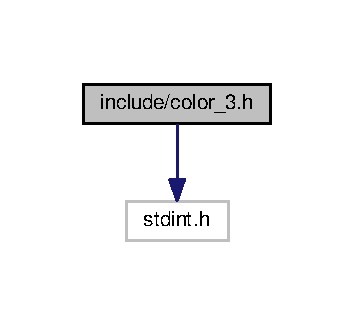
\includegraphics[width=170pt]{color__3_8h__incl}
\end{center}
\end{figure}
This graph shows which files directly or indirectly include this file\+:
\nopagebreak
\begin{figure}[H]
\begin{center}
\leavevmode
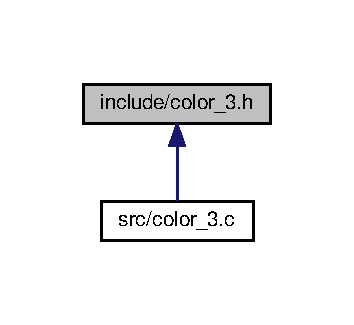
\includegraphics[width=170pt]{color__3_8h__dep__incl}
\end{center}
\end{figure}
\subsection*{Data Structures}
\begin{DoxyCompactItemize}
\item 
struct \hyperlink{structcolor__t}{color\+\_\+t}
\end{DoxyCompactItemize}
\subsection*{Functions}
\begin{DoxyCompactItemize}
\item 
void \hyperlink{color__3_8h_a9f116bb54a359aae1dcbc3397be95005}{color\+\_\+3\+\_\+init} (uint8\+\_\+t address)
\item 
void \hyperlink{color__3_8h_a160121e4bf056da0e86f7ba476547335}{color\+\_\+3\+\_\+get\+\_\+rgb\+\_\+data} (\hyperlink{structcolor__t}{color\+\_\+t} $\ast$color)
\end{DoxyCompactItemize}


\subsection{Detailed Description}
Color 3 click. 

\begin{DoxyAuthor}{Author}
Mikro\+Elektronika Team 
\end{DoxyAuthor}
\begin{DoxyDate}{Date}
04/10/16
\end{DoxyDate}
\begin{DoxyParagraph}{}
Functions set for Color 3.
\end{DoxyParagraph}
\begin{DoxyVersion}{Version}

\begin{DoxyItemize}
\item 1.\+0.\+0 Initial version
\item 1.\+0.\+1 Doxy added ( Color 3 )
\end{DoxyItemize}
\end{DoxyVersion}
\begin{DoxyParagraph}{}
\href{../datasheet/color_3.pdf}{\tt Datasheet}
\end{DoxyParagraph}
\begin{DoxyCopyright}{Copyright}
\subparagraph*{\href{../../COPYING}{\tt G\+N\+U G\+P\+L 2}}
\end{DoxyCopyright}


\subsection{Function Documentation}
\hypertarget{color__3_8h_a160121e4bf056da0e86f7ba476547335}{}\index{color\+\_\+3.\+h@{color\+\_\+3.\+h}!color\+\_\+3\+\_\+get\+\_\+rgb\+\_\+data@{color\+\_\+3\+\_\+get\+\_\+rgb\+\_\+data}}
\index{color\+\_\+3\+\_\+get\+\_\+rgb\+\_\+data@{color\+\_\+3\+\_\+get\+\_\+rgb\+\_\+data}!color\+\_\+3.\+h@{color\+\_\+3.\+h}}
\subsubsection[{color\+\_\+3\+\_\+get\+\_\+rgb\+\_\+data}]{\setlength{\rightskip}{0pt plus 5cm}void color\+\_\+3\+\_\+get\+\_\+rgb\+\_\+data (
\begin{DoxyParamCaption}
\item[{{\bf color\+\_\+t} $\ast$}]{color}
\end{DoxyParamCaption}
)}\label{color__3_8h_a160121e4bf056da0e86f7ba476547335}
\paragraph*{Color 3 Get R\+G\+B Data }

\begin{DoxyParagraph}{}
Gets clear, red, green, and blue data from click.
\end{DoxyParagraph}

\begin{DoxyParams}[1]{Parameters}
\mbox{\tt in}  & {\em color} & -\/ \hyperlink{structcolor__t}{color\+\_\+t} struct for returning clear and rgb data. \\
\hline
\end{DoxyParams}
\hypertarget{color__3_8h_a9f116bb54a359aae1dcbc3397be95005}{}\index{color\+\_\+3.\+h@{color\+\_\+3.\+h}!color\+\_\+3\+\_\+init@{color\+\_\+3\+\_\+init}}
\index{color\+\_\+3\+\_\+init@{color\+\_\+3\+\_\+init}!color\+\_\+3.\+h@{color\+\_\+3.\+h}}
\subsubsection[{color\+\_\+3\+\_\+init}]{\setlength{\rightskip}{0pt plus 5cm}void color\+\_\+3\+\_\+init (
\begin{DoxyParamCaption}
\item[{uint8\+\_\+t}]{address}
\end{DoxyParamCaption}
)}\label{color__3_8h_a9f116bb54a359aae1dcbc3397be95005}
\paragraph*{Color 3 Initialization }

\begin{DoxyParagraph}{}
Initializes Color 3
\end{DoxyParagraph}
\begin{DoxyNote}{Note}
This function must be called first. 
\end{DoxyNote}

\hypertarget{color__3__hal_8h}{}\section{include/color\+\_\+3\+\_\+hal.h File Reference}
\label{color__3__hal_8h}\index{include/color\+\_\+3\+\_\+hal.\+h@{include/color\+\_\+3\+\_\+hal.\+h}}
{\ttfamily \#include $<$stdint.\+h$>$}\\*
Include dependency graph for color\+\_\+3\+\_\+hal.\+h\+:
\nopagebreak
\begin{figure}[H]
\begin{center}
\leavevmode
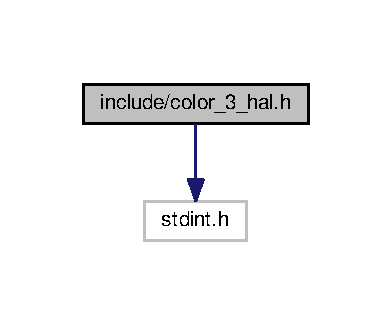
\includegraphics[width=188pt]{color__3__hal_8h__incl}
\end{center}
\end{figure}
This graph shows which files directly or indirectly include this file\+:
\nopagebreak
\begin{figure}[H]
\begin{center}
\leavevmode
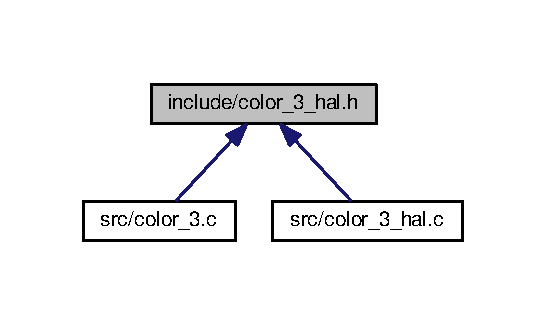
\includegraphics[width=262pt]{color__3__hal_8h__dep__incl}
\end{center}
\end{figure}
\subsection*{Macros}
\begin{DoxyCompactItemize}
\item 
\hypertarget{color__3__hal_8h_ab991bcb3e9d7f3503ef001b546205e5b}{}\#define {\bfseries T\+C\+S3771\+\_\+\+C\+O\+M\+M\+A\+N\+D\+\_\+\+T\+Y\+P\+E\+\_\+\+S\+P\+E\+C\+I\+A\+L}~(3 $<$$<$ 5)\label{color__3__hal_8h_ab991bcb3e9d7f3503ef001b546205e5b}

\item 
\hypertarget{color__3__hal_8h_aac838b683c94c07d0b84c4bdb90c00bd}{}\#define {\bfseries T\+C\+S3771\+\_\+\+C\+O\+M\+M\+A\+N\+D\+\_\+\+T\+Y\+P\+E\+\_\+\+A\+U\+T\+O\+I\+N\+C}~(0b01 $<$$<$ 5)\label{color__3__hal_8h_aac838b683c94c07d0b84c4bdb90c00bd}

\item 
\hypertarget{color__3__hal_8h_ad1455e9122a371f341eeb9c60bd80968}{}\#define {\bfseries T\+C\+S3771\+\_\+\+C\+O\+M\+M\+A\+N\+D\+\_\+\+S\+E\+L\+E\+C\+T}~(1 $<$$<$ 7)\label{color__3__hal_8h_ad1455e9122a371f341eeb9c60bd80968}

\end{DoxyCompactItemize}
\subsection*{Enumerations}
\begin{DoxyCompactItemize}
\item 
\hypertarget{color__3__hal_8h_a07a6a91973814c0c577756f699c1e34b}{}enum {\bfseries cmd\+\_\+type\+\_\+t} \{ {\bfseries S\+P\+E\+C\+I\+A\+L\+\_\+\+T\+Y\+P\+E} = 0, 
{\bfseries N\+O\+R\+M\+A\+L\+\_\+\+T\+Y\+P\+E} = 1
 \}\label{color__3__hal_8h_a07a6a91973814c0c577756f699c1e34b}

\end{DoxyCompactItemize}
\subsection*{Functions}
\begin{DoxyCompactItemize}
\item 
void \hyperlink{color__3__hal_8h_a1eb89db63de5f77f2a34c42e5a353d91}{color\+\_\+3\+\_\+hal\+\_\+init} (uint8\+\_\+t address\+\_\+id, uint8\+\_\+t command\+\_\+size)
\item 
void \hyperlink{color__3__hal_8h_ae1d223178a020ecf9b22a21760b12bc9}{color\+\_\+3\+\_\+hal\+\_\+write} (uint8\+\_\+t $\ast$buffer, uint8\+\_\+t reg, uint16\+\_\+t count, cmd\+\_\+type\+\_\+t type)
\item 
void \hyperlink{color__3__hal_8h_a462e1e44613feefb21f65a6cb23b784a}{color\+\_\+3\+\_\+hal\+\_\+read} (uint8\+\_\+t $\ast$buffer, uint8\+\_\+t reg, uint8\+\_\+t count)
\end{DoxyCompactItemize}


\subsection{Detailed Description}
\subsubsection*{H\+A\+L layer }

\subsection{Function Documentation}
\hypertarget{color__3__hal_8h_a1eb89db63de5f77f2a34c42e5a353d91}{}\index{color\+\_\+3\+\_\+hal.\+h@{color\+\_\+3\+\_\+hal.\+h}!color\+\_\+3\+\_\+hal\+\_\+init@{color\+\_\+3\+\_\+hal\+\_\+init}}
\index{color\+\_\+3\+\_\+hal\+\_\+init@{color\+\_\+3\+\_\+hal\+\_\+init}!color\+\_\+3\+\_\+hal.\+h@{color\+\_\+3\+\_\+hal.\+h}}
\subsubsection[{color\+\_\+3\+\_\+hal\+\_\+init}]{\setlength{\rightskip}{0pt plus 5cm}void color\+\_\+3\+\_\+hal\+\_\+init (
\begin{DoxyParamCaption}
\item[{uint8\+\_\+t}]{address\+\_\+id, }
\item[{uint8\+\_\+t}]{command\+\_\+size}
\end{DoxyParamCaption}
)}\label{color__3__hal_8h_a1eb89db63de5f77f2a34c42e5a353d91}
\paragraph*{H\+A\+L Initialization}

\begin{DoxyParagraph}{}
Initialization of H\+A\+L layer used to initialize I2\+C bus and pins needed for proper usage of click board.
\end{DoxyParagraph}

\begin{DoxyParams}[1]{Parameters}
\mbox{\tt in}  & {\em address\+\_\+id} & -\/ hardware address \\
\hline
\end{DoxyParams}
\hypertarget{color__3__hal_8h_a462e1e44613feefb21f65a6cb23b784a}{}\index{color\+\_\+3\+\_\+hal.\+h@{color\+\_\+3\+\_\+hal.\+h}!color\+\_\+3\+\_\+hal\+\_\+read@{color\+\_\+3\+\_\+hal\+\_\+read}}
\index{color\+\_\+3\+\_\+hal\+\_\+read@{color\+\_\+3\+\_\+hal\+\_\+read}!color\+\_\+3\+\_\+hal.\+h@{color\+\_\+3\+\_\+hal.\+h}}
\subsubsection[{color\+\_\+3\+\_\+hal\+\_\+read}]{\setlength{\rightskip}{0pt plus 5cm}void color\+\_\+3\+\_\+hal\+\_\+read (
\begin{DoxyParamCaption}
\item[{uint8\+\_\+t $\ast$}]{buffer, }
\item[{uint8\+\_\+t}]{reg, }
\item[{uint8\+\_\+t}]{count}
\end{DoxyParamCaption}
)}\label{color__3__hal_8h_a462e1e44613feefb21f65a6cb23b784a}
\paragraph*{H\+A\+L Read}

\begin{DoxyParagraph}{}
Generic read function adapted for color\+\_\+3 click.
\end{DoxyParagraph}
\begin{DoxyNote}{Note}
Buffer caries command which will be rewritten after reading.
\end{DoxyNote}

\begin{DoxyParams}{Parameters}
{\em } & \\
\hline
\end{DoxyParams}
\hypertarget{color__3__hal_8h_ae1d223178a020ecf9b22a21760b12bc9}{}\index{color\+\_\+3\+\_\+hal.\+h@{color\+\_\+3\+\_\+hal.\+h}!color\+\_\+3\+\_\+hal\+\_\+write@{color\+\_\+3\+\_\+hal\+\_\+write}}
\index{color\+\_\+3\+\_\+hal\+\_\+write@{color\+\_\+3\+\_\+hal\+\_\+write}!color\+\_\+3\+\_\+hal.\+h@{color\+\_\+3\+\_\+hal.\+h}}
\subsubsection[{color\+\_\+3\+\_\+hal\+\_\+write}]{\setlength{\rightskip}{0pt plus 5cm}void color\+\_\+3\+\_\+hal\+\_\+write (
\begin{DoxyParamCaption}
\item[{uint8\+\_\+t $\ast$}]{buffer, }
\item[{uint8\+\_\+t}]{reg, }
\item[{uint16\+\_\+t}]{count, }
\item[{cmd\+\_\+type\+\_\+t}]{type}
\end{DoxyParamCaption}
)}\label{color__3__hal_8h_ae1d223178a020ecf9b22a21760b12bc9}
\paragraph*{H\+A\+L Write}

\begin{DoxyParagraph}{}
Generic write function adapted for color\+\_\+3 click.
\end{DoxyParagraph}

\begin{DoxyParams}[1]{Parameters}
\mbox{\tt in}  & {\em buffer} & -\/ data buffer \\
\hline
\mbox{\tt in}  & {\em count} & -\/ data size in bytes \\
\hline
\end{DoxyParams}

\hypertarget{color__3_8c}{}\section{src/color\+\_\+3.c File Reference}
\label{color__3_8c}\index{src/color\+\_\+3.\+c@{src/color\+\_\+3.\+c}}


Color 3 click.  


{\ttfamily \#include \char`\"{}color\+\_\+3.\+h\char`\"{}}\\*
{\ttfamily \#include \char`\"{}color\+\_\+3\+\_\+hal.\+h\char`\"{}}\\*
Include dependency graph for color\+\_\+3.\+c\+:
\nopagebreak
\begin{figure}[H]
\begin{center}
\leavevmode
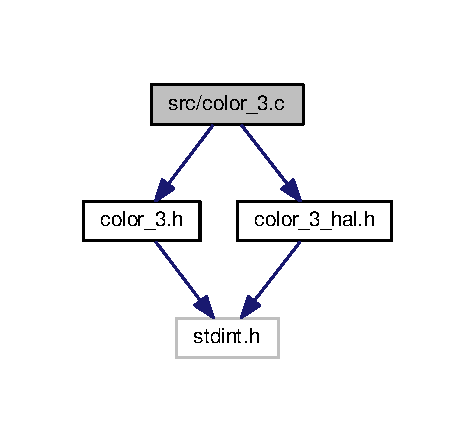
\includegraphics[width=228pt]{color__3_8c__incl}
\end{center}
\end{figure}
\subsection*{Macros}
\begin{DoxyCompactItemize}
\item 
\hypertarget{color__3_8c_ab991bcb3e9d7f3503ef001b546205e5b}{}\#define {\bfseries T\+C\+S3771\+\_\+\+C\+O\+M\+M\+A\+N\+D\+\_\+\+T\+Y\+P\+E\+\_\+\+S\+P\+E\+C\+I\+A\+L}~(3 $<$$<$ 5)\label{color__3_8c_ab991bcb3e9d7f3503ef001b546205e5b}

\item 
\hypertarget{color__3_8c_aac838b683c94c07d0b84c4bdb90c00bd}{}\#define {\bfseries T\+C\+S3771\+\_\+\+C\+O\+M\+M\+A\+N\+D\+\_\+\+T\+Y\+P\+E\+\_\+\+A\+U\+T\+O\+I\+N\+C}~(0b01 $<$$<$ 5)\label{color__3_8c_aac838b683c94c07d0b84c4bdb90c00bd}

\item 
\hypertarget{color__3_8c_ad1455e9122a371f341eeb9c60bd80968}{}\#define {\bfseries T\+C\+S3771\+\_\+\+C\+O\+M\+M\+A\+N\+D\+\_\+\+S\+E\+L\+E\+C\+T}~(1 $<$$<$ 7)\label{color__3_8c_ad1455e9122a371f341eeb9c60bd80968}

\item 
\hypertarget{color__3_8c_ace3d5257e08d409a706ed4222e8c355e}{}\#define {\bfseries T\+C\+S3771\+\_\+\+E\+N\+A\+B\+L\+E}~0x00\label{color__3_8c_ace3d5257e08d409a706ed4222e8c355e}

\item 
\hypertarget{color__3_8c_a58829c5fc039c072070018b4b2b2c1a5}{}\#define {\bfseries T\+C\+S3771\+\_\+\+E\+N\+A\+B\+L\+E\+\_\+\+P\+O\+N}~(1 $<$$<$ 0)\label{color__3_8c_a58829c5fc039c072070018b4b2b2c1a5}

\item 
\hypertarget{color__3_8c_a16e2275711da55fcf5c5274c79427080}{}\#define {\bfseries T\+C\+S3771\+\_\+\+E\+N\+A\+B\+L\+E\+\_\+\+A\+E\+N}~(1 $<$$<$ 1)\label{color__3_8c_a16e2275711da55fcf5c5274c79427080}

\item 
\hypertarget{color__3_8c_a0e4a24993bb9aa7bd1c8b6f6c60c7a9c}{}\#define {\bfseries T\+C\+S3771\+\_\+\+E\+N\+A\+B\+L\+E\+\_\+\+P\+E\+N}~(1 $<$$<$ 2)\label{color__3_8c_a0e4a24993bb9aa7bd1c8b6f6c60c7a9c}

\item 
\hypertarget{color__3_8c_a3ba0727605ad60b2cdd22f85ce42d867}{}\#define {\bfseries T\+C\+S3771\+\_\+\+E\+N\+A\+B\+L\+E\+\_\+\+W\+E\+N}~(1 $<$$<$ 3)\label{color__3_8c_a3ba0727605ad60b2cdd22f85ce42d867}

\item 
\hypertarget{color__3_8c_ac7439a0712ad950c132a0d158819d010}{}\#define {\bfseries T\+C\+S3771\+\_\+\+E\+N\+A\+B\+L\+E\+\_\+\+A\+I\+E\+N}~(1 $<$$<$ 4)\label{color__3_8c_ac7439a0712ad950c132a0d158819d010}

\item 
\hypertarget{color__3_8c_a4c4676190175cafae89b3bceaa2889df}{}\#define {\bfseries T\+C\+S3771\+\_\+\+E\+N\+A\+B\+L\+E\+\_\+\+P\+I\+E\+N}~(1 $<$$<$ 5)\label{color__3_8c_a4c4676190175cafae89b3bceaa2889df}

\item 
\hypertarget{color__3_8c_a102a4bd37f8702f783562f3ee7d3f37f}{}\#define {\bfseries T\+C\+S3771\+\_\+\+A\+T\+I\+M\+E}~0x01\label{color__3_8c_a102a4bd37f8702f783562f3ee7d3f37f}

\item 
\hypertarget{color__3_8c_a233500a3f78df902307a0fd1f4633cf5}{}\#define {\bfseries T\+C\+S3771\+\_\+\+P\+T\+I\+M\+E}~0x02\label{color__3_8c_a233500a3f78df902307a0fd1f4633cf5}

\item 
\hypertarget{color__3_8c_aaef8ecbe3e65e65d657047840927f5cd}{}\#define {\bfseries T\+C\+S3771\+\_\+\+W\+T\+I\+M\+E}~0x03\label{color__3_8c_aaef8ecbe3e65e65d657047840927f5cd}

\item 
\hypertarget{color__3_8c_a9cf2ef509a538f6989d8d12a243ac641}{}\#define {\bfseries T\+C\+S3771\+\_\+\+A\+I\+L\+T}~0x04\label{color__3_8c_a9cf2ef509a538f6989d8d12a243ac641}

\item 
\hypertarget{color__3_8c_a0dd9b9b76e3a4abb1649e142d897bdf4}{}\#define {\bfseries T\+C\+S3771\+\_\+\+A\+I\+H\+T}~0x06\label{color__3_8c_a0dd9b9b76e3a4abb1649e142d897bdf4}

\item 
\hypertarget{color__3_8c_a51a8e34c2fdd1265d1951252a0cb8293}{}\#define {\bfseries T\+C\+S3771\+\_\+\+P\+I\+L\+T}~0x08\label{color__3_8c_a51a8e34c2fdd1265d1951252a0cb8293}

\item 
\hypertarget{color__3_8c_a79b1cda6326a92a76d1088a0cb3100ea}{}\#define {\bfseries T\+C\+S3771\+\_\+\+P\+I\+H\+T}~0x0a\label{color__3_8c_a79b1cda6326a92a76d1088a0cb3100ea}

\item 
\hypertarget{color__3_8c_ad1946a77ac5243562462cde439cec8be}{}\#define {\bfseries T\+C\+S3771\+\_\+\+P\+E\+R\+S}~0x0c\label{color__3_8c_ad1946a77ac5243562462cde439cec8be}

\item 
\hypertarget{color__3_8c_a0ab498632a829eaa170e5fbeb188d6ef}{}\#define {\bfseries T\+C\+S3771\+\_\+\+P\+E\+R\+S\+\_\+\+P\+P\+E\+R\+S}(x)~((x) $<$$<$ 4)\label{color__3_8c_a0ab498632a829eaa170e5fbeb188d6ef}

\item 
\hypertarget{color__3_8c_a7ae44a8dcbc7c40e9171839bba292549}{}\#define {\bfseries T\+C\+S3771\+\_\+\+P\+E\+R\+S\+\_\+\+A\+P\+E\+R\+S}(x)~((x) \& 0xf)\label{color__3_8c_a7ae44a8dcbc7c40e9171839bba292549}

\item 
\hypertarget{color__3_8c_a53180239013e855a2013f4891c4bada1}{}\#define {\bfseries T\+C\+S3771\+\_\+\+C\+O\+N\+F}~0x0d\label{color__3_8c_a53180239013e855a2013f4891c4bada1}

\item 
\hypertarget{color__3_8c_ae9cf122497fdd904f7e473701e1f9364}{}\#define {\bfseries T\+C\+S3771\+\_\+\+C\+O\+N\+F\+\_\+\+W\+L\+O\+N\+G}~(1 $<$$<$ 1)\label{color__3_8c_ae9cf122497fdd904f7e473701e1f9364}

\item 
\hypertarget{color__3_8c_adf08fa94f2ae46b0efee8f4a25fb4840}{}\#define {\bfseries T\+C\+S3771\+\_\+\+P\+P\+U\+L\+S\+E}~0x0e\label{color__3_8c_adf08fa94f2ae46b0efee8f4a25fb4840}

\item 
\hypertarget{color__3_8c_a7581b03d138efb10438ada58da112836}{}\#define {\bfseries T\+C\+S3771\+\_\+\+C\+O\+N\+T\+R\+O\+L}~0x0f\label{color__3_8c_a7581b03d138efb10438ada58da112836}

\item 
\hypertarget{color__3_8c_a55d4b7c7a8f3ed5979b6f67b401d4ae8}{}\#define {\bfseries T\+C\+S3771\+\_\+\+C\+O\+N\+T\+R\+O\+L\+\_\+\+P\+D\+I\+O\+D\+E\+\_\+\+I\+R}~(0b10 $<$$<$ 4)\label{color__3_8c_a55d4b7c7a8f3ed5979b6f67b401d4ae8}

\item 
\hypertarget{color__3_8c_a04d9f9aadce6d6481162b9cb566ce72a}{}\#define {\bfseries T\+C\+S3771\+\_\+\+I\+D}~0x12\label{color__3_8c_a04d9f9aadce6d6481162b9cb566ce72a}

\item 
\hypertarget{color__3_8c_a78dbd9fe90c44cd903da291e9246fe1a}{}\#define {\bfseries T\+C\+S3771\+\_\+\+S\+T\+A\+T\+U\+S}~0x13\label{color__3_8c_a78dbd9fe90c44cd903da291e9246fe1a}

\item 
\hypertarget{color__3_8c_a01787401b2da60ea96a88da301ff9adc}{}\#define {\bfseries T\+C\+S3771\+\_\+\+P\+D\+A\+T\+A}~0x1c\label{color__3_8c_a01787401b2da60ea96a88da301ff9adc}

\item 
\hypertarget{color__3_8c_a5f0662fd0e765faccbb6d02c15a76538}{}\#define {\bfseries T\+C\+S3771\+\_\+\+C\+D\+A\+T\+A}~0x14\label{color__3_8c_a5f0662fd0e765faccbb6d02c15a76538}

\end{DoxyCompactItemize}
\subsection*{Functions}
\begin{DoxyCompactItemize}
\item 
void \hyperlink{color__3_8c_a9f116bb54a359aae1dcbc3397be95005}{color\+\_\+3\+\_\+init} (uint8\+\_\+t address)
\item 
void \hyperlink{color__3_8c_a160121e4bf056da0e86f7ba476547335}{color\+\_\+3\+\_\+get\+\_\+rgb\+\_\+data} (\hyperlink{structcolor__t}{color\+\_\+t} $\ast$color)
\end{DoxyCompactItemize}


\subsection{Detailed Description}
Color 3 click. 

\begin{DoxyAuthor}{Author}
Mikro\+Elektronika Team 
\end{DoxyAuthor}
\begin{DoxyDate}{Date}
04/10/16
\end{DoxyDate}
\begin{DoxyParagraph}{}
Functions set for Color 3.
\end{DoxyParagraph}
\begin{DoxyVersion}{Version}

\begin{DoxyItemize}
\item 1.\+0.\+0 Initial version
\item 1.\+0.\+1 Doxy added ( Color 3 )
\end{DoxyItemize}
\end{DoxyVersion}
\begin{DoxyParagraph}{}
\href{../datasheet/color_3.pdf}{\tt Datasheet}
\end{DoxyParagraph}
\begin{DoxyCopyright}{Copyright}
\subparagraph*{\href{../../COPYING}{\tt G\+N\+U G\+P\+L 2}}
\end{DoxyCopyright}


\subsection{Function Documentation}
\hypertarget{color__3_8c_a160121e4bf056da0e86f7ba476547335}{}\index{color\+\_\+3.\+c@{color\+\_\+3.\+c}!color\+\_\+3\+\_\+get\+\_\+rgb\+\_\+data@{color\+\_\+3\+\_\+get\+\_\+rgb\+\_\+data}}
\index{color\+\_\+3\+\_\+get\+\_\+rgb\+\_\+data@{color\+\_\+3\+\_\+get\+\_\+rgb\+\_\+data}!color\+\_\+3.\+c@{color\+\_\+3.\+c}}
\subsubsection[{color\+\_\+3\+\_\+get\+\_\+rgb\+\_\+data}]{\setlength{\rightskip}{0pt plus 5cm}void color\+\_\+3\+\_\+get\+\_\+rgb\+\_\+data (
\begin{DoxyParamCaption}
\item[{{\bf color\+\_\+t} $\ast$}]{color}
\end{DoxyParamCaption}
)}\label{color__3_8c_a160121e4bf056da0e86f7ba476547335}
\paragraph*{Color 3 Get R\+G\+B Data }

\begin{DoxyParagraph}{}
Gets clear, red, green, and blue data from click.
\end{DoxyParagraph}

\begin{DoxyParams}[1]{Parameters}
\mbox{\tt in}  & {\em color} & -\/ \hyperlink{structcolor__t}{color\+\_\+t} struct for returning clear and rgb data. \\
\hline
\end{DoxyParams}
\hypertarget{color__3_8c_a9f116bb54a359aae1dcbc3397be95005}{}\index{color\+\_\+3.\+c@{color\+\_\+3.\+c}!color\+\_\+3\+\_\+init@{color\+\_\+3\+\_\+init}}
\index{color\+\_\+3\+\_\+init@{color\+\_\+3\+\_\+init}!color\+\_\+3.\+c@{color\+\_\+3.\+c}}
\subsubsection[{color\+\_\+3\+\_\+init}]{\setlength{\rightskip}{0pt plus 5cm}void color\+\_\+3\+\_\+init (
\begin{DoxyParamCaption}
\item[{uint8\+\_\+t}]{address}
\end{DoxyParamCaption}
)}\label{color__3_8c_a9f116bb54a359aae1dcbc3397be95005}
\paragraph*{Color 3 Initialization }

\begin{DoxyParagraph}{}
Initializes Color 3
\end{DoxyParagraph}
\begin{DoxyNote}{Note}
This function must be called first. 
\end{DoxyNote}

\hypertarget{color__3__hal_8c}{}\section{src/color\+\_\+3\+\_\+hal.c File Reference}
\label{color__3__hal_8c}\index{src/color\+\_\+3\+\_\+hal.\+c@{src/color\+\_\+3\+\_\+hal.\+c}}
{\ttfamily \#include \char`\"{}color\+\_\+3\+\_\+hal.\+h\char`\"{}}\\*
Include dependency graph for color\+\_\+3\+\_\+hal.\+c\+:
\nopagebreak
\begin{figure}[H]
\begin{center}
\leavevmode
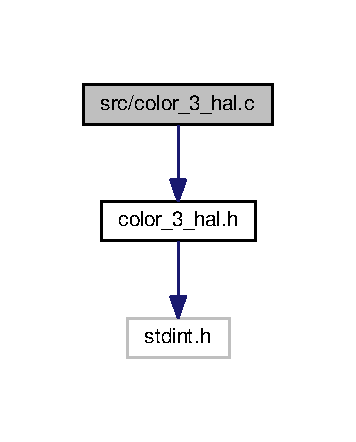
\includegraphics[width=171pt]{color__3__hal_8c__incl}
\end{center}
\end{figure}
\subsection*{Macros}
\begin{DoxyCompactItemize}
\item 
\hypertarget{color__3__hal_8c_a2f493ed233e66342493f155ebda5c183}{}\#define {\bfseries R\+E\+A\+D\+\_\+\+B\+I\+T}~1\label{color__3__hal_8c_a2f493ed233e66342493f155ebda5c183}

\item 
\hypertarget{color__3__hal_8c_a7fc57d5be9f588839a00c75ef2946e17}{}\#define {\bfseries W\+R\+I\+T\+E\+\_\+\+B\+I\+T}~0\label{color__3__hal_8c_a7fc57d5be9f588839a00c75ef2946e17}

\item 
\hypertarget{color__3__hal_8c_a27fd8f8401ebd63d438cc642eb130749}{}\#define {\bfseries \+\_\+\+\_\+\+A\+T\+M\+E\+G\+A\+\_\+\+\_\+}\label{color__3__hal_8c_a27fd8f8401ebd63d438cc642eb130749}

\end{DoxyCompactItemize}
\subsection*{Functions}
\begin{DoxyCompactItemize}
\item 
void \hyperlink{color__3__hal_8c_a1eb89db63de5f77f2a34c42e5a353d91}{color\+\_\+3\+\_\+hal\+\_\+init} (uint8\+\_\+t address\+\_\+id, uint8\+\_\+t command\+\_\+size)
\item 
void \hyperlink{color__3__hal_8c_ae1d223178a020ecf9b22a21760b12bc9}{color\+\_\+3\+\_\+hal\+\_\+write} (uint8\+\_\+t $\ast$buffer, uint8\+\_\+t reg, uint16\+\_\+t count, cmd\+\_\+type\+\_\+t type)
\item 
void \hyperlink{color__3__hal_8c_a462e1e44613feefb21f65a6cb23b784a}{color\+\_\+3\+\_\+hal\+\_\+read} (uint8\+\_\+t $\ast$buffer, uint8\+\_\+t reg, uint8\+\_\+t count)
\end{DoxyCompactItemize}


\subsection{Detailed Description}
\subsubsection*{H\+A\+L layer }

\subsection{Function Documentation}
\hypertarget{color__3__hal_8c_a1eb89db63de5f77f2a34c42e5a353d91}{}\index{color\+\_\+3\+\_\+hal.\+c@{color\+\_\+3\+\_\+hal.\+c}!color\+\_\+3\+\_\+hal\+\_\+init@{color\+\_\+3\+\_\+hal\+\_\+init}}
\index{color\+\_\+3\+\_\+hal\+\_\+init@{color\+\_\+3\+\_\+hal\+\_\+init}!color\+\_\+3\+\_\+hal.\+c@{color\+\_\+3\+\_\+hal.\+c}}
\subsubsection[{color\+\_\+3\+\_\+hal\+\_\+init}]{\setlength{\rightskip}{0pt plus 5cm}void color\+\_\+3\+\_\+hal\+\_\+init (
\begin{DoxyParamCaption}
\item[{uint8\+\_\+t}]{address\+\_\+id, }
\item[{uint8\+\_\+t}]{command\+\_\+size}
\end{DoxyParamCaption}
)}\label{color__3__hal_8c_a1eb89db63de5f77f2a34c42e5a353d91}
\paragraph*{H\+A\+L Initialization}

\begin{DoxyParagraph}{}
Initialization of H\+A\+L layer used to initialize I2\+C bus and pins needed for proper usage of click board.
\end{DoxyParagraph}

\begin{DoxyParams}[1]{Parameters}
\mbox{\tt in}  & {\em address\+\_\+id} & -\/ hardware address \\
\hline
\end{DoxyParams}
\hypertarget{color__3__hal_8c_a462e1e44613feefb21f65a6cb23b784a}{}\index{color\+\_\+3\+\_\+hal.\+c@{color\+\_\+3\+\_\+hal.\+c}!color\+\_\+3\+\_\+hal\+\_\+read@{color\+\_\+3\+\_\+hal\+\_\+read}}
\index{color\+\_\+3\+\_\+hal\+\_\+read@{color\+\_\+3\+\_\+hal\+\_\+read}!color\+\_\+3\+\_\+hal.\+c@{color\+\_\+3\+\_\+hal.\+c}}
\subsubsection[{color\+\_\+3\+\_\+hal\+\_\+read}]{\setlength{\rightskip}{0pt plus 5cm}void color\+\_\+3\+\_\+hal\+\_\+read (
\begin{DoxyParamCaption}
\item[{uint8\+\_\+t $\ast$}]{buffer, }
\item[{uint8\+\_\+t}]{reg, }
\item[{uint8\+\_\+t}]{count}
\end{DoxyParamCaption}
)}\label{color__3__hal_8c_a462e1e44613feefb21f65a6cb23b784a}
\paragraph*{H\+A\+L Read}

\begin{DoxyParagraph}{}
Generic read function adapted for color\+\_\+3 click.
\end{DoxyParagraph}
\begin{DoxyNote}{Note}
Buffer caries command which will be rewritten after reading.
\end{DoxyNote}

\begin{DoxyParams}{Parameters}
{\em } & \\
\hline
\end{DoxyParams}
\hypertarget{color__3__hal_8c_ae1d223178a020ecf9b22a21760b12bc9}{}\index{color\+\_\+3\+\_\+hal.\+c@{color\+\_\+3\+\_\+hal.\+c}!color\+\_\+3\+\_\+hal\+\_\+write@{color\+\_\+3\+\_\+hal\+\_\+write}}
\index{color\+\_\+3\+\_\+hal\+\_\+write@{color\+\_\+3\+\_\+hal\+\_\+write}!color\+\_\+3\+\_\+hal.\+c@{color\+\_\+3\+\_\+hal.\+c}}
\subsubsection[{color\+\_\+3\+\_\+hal\+\_\+write}]{\setlength{\rightskip}{0pt plus 5cm}void color\+\_\+3\+\_\+hal\+\_\+write (
\begin{DoxyParamCaption}
\item[{uint8\+\_\+t $\ast$}]{buffer, }
\item[{uint8\+\_\+t}]{reg, }
\item[{uint16\+\_\+t}]{count, }
\item[{cmd\+\_\+type\+\_\+t}]{type}
\end{DoxyParamCaption}
)}\label{color__3__hal_8c_ae1d223178a020ecf9b22a21760b12bc9}
\paragraph*{H\+A\+L Write}

\begin{DoxyParagraph}{}
Generic write function adapted for color\+\_\+3 click.
\end{DoxyParagraph}

\begin{DoxyParams}[1]{Parameters}
\mbox{\tt in}  & {\em buffer} & -\/ data buffer \\
\hline
\mbox{\tt in}  & {\em count} & -\/ data size in bytes \\
\hline
\end{DoxyParams}

%--- End generated contents ---

% Index
\backmatter
\newpage
\phantomsection
\clearemptydoublepage
\addcontentsline{toc}{chapter}{Index}
\printindex

\end{document}
